\levelstay{Brownian Motion in a Plane}

\leveldown{Problem}

Use solution $X(t) = N^t_{0,x}(0,1)\sqrt{\delta^2 t}$ and $Y(t) = N^t_{0,y}(0,1)\sqrt{\delta^2 t}$ and the method in section 6.4 to generate and plot a Brownian particle sample path in the x-y plane.
Assume the unit normals $N^t_{0,x}$ and $N^t_{0,y}$ (and thus displacements in the two directions) are statistically independent.

\levelstay{Solution}

We use the following code, which can be found in the following code listing:

\lstinputlisting[frame=single]{random_walk_2d.py}

An example output is shown in Figure \ref{Fig:ch6.problem4.2drandomwalk}.

\begin{figure}
  \begin{centering}
  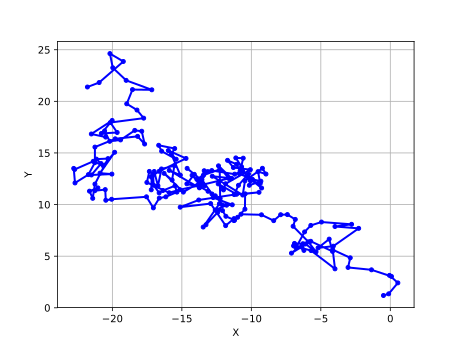
\includegraphics[width=0.9\textwidth]{random_walk_2d.pdf}
  \par\end{centering}
  \caption{A two dimensional random walk}
  \label{Fig:ch6.problem4.2drandomwalk}
\end{figure}
